\documentclass{beamer}
\usepackage{amsmath}
\usepackage{amsthm}
\usepackage{amssymb}
\usepackage{amsfonts}
\usepackage[mathscr]{euscript}
\usepackage{tikz}
\usepackage{tikz-cd}
\usepackage{beamerthemeshadow}
%\usepackage[absolute]{textpos}
\usepackage[absolute, overlay]{textpos}
\usepackage{wrapfig}
\usepackage{caption}
\usepackage{dirtytalk}
\usepackage{graphicx}
\usepackage{subcaption}
% \usepackage{movie15}
% \usepackage{animate}
\usetikzlibrary{decorations.pathmorphing,shapes}


\usepackage{bbold}
\usepackage[bbgreekl]{mathbbol}


\captionsetup[figure]{name=}

\tikzset{
	invisible/.style={opacity=0},
	visible on/.style={alt={#1{}{invisible}}},
	alt/.code args={<#1>#2#3}{%
		\alt<#1>{\pgfkeysalso{#2}}{\pgfkeysalso{#3}}%
	}
}


%\newcommand{\bbefamily}{\fontencoding{U}\fontfamily{bbold}\selectfont}
%\newcommand{\textbbe}[1]{{\bbefamily #1}}
%\DeclareMathAlphabet{\mathbbe}{U}{bbold}{m}{n}
%
%\def\DDelta{{\mathbbe{\Delta}}}
%
%\newcommand{\DD}{\DDelta}


\newcommand{\B}{\mathscr{B}}
\newcommand{\C}{\mathscr{C}}
\newcommand{\D}{\mathscr{D}}
\newcommand{\cO}{\mathscr{O}}
\newcommand{\M}{\mathscr{M}}
\newcommand{\s}{\mathscr{S}}
\newcommand{\set}{\mathscr{S}\mathrm{et}}
\newcommand{\sSet}{\mathrm{s}\mathscr{S}\mathrm{et}}
\newcommand{\cat}{\mathscr{C}\mathrm{at}}
\newcommand{\twocat}{2\mathscr{C}\mathrm{at}}
\newcommand{\bicat}{\mathrm{bi}\mathscr{C}\mathrm{at}}
\newcommand{\id}{\mathrm{id}}
\newcommand{\Univ}{\mathscr{U}\mathrm{niv}}
\newcommand{\HH}{\mathrm{HH}}
\newcommand{\THH}{\mathrm{THH}}
\newcommand{\Fun}{\mathrm{Fun}}
\newcommand{\Pic}{\mathrm{Pic}}
\newcommand{\Mod}{\mathrm{Mod}}
\newcommand{\Sp}{\mathrm{Sp}}
\newcommand{\ds}{\displaystyle}
\newcommand{\sma}{\wedge}

\expandafter\def\expandafter\insertshorttitle\expandafter{%
  \insertshorttitle\hfill\insertframenumber\,/\,\inserttotalframenumber}

\setbeamertemplate{navigation symbols}{}

\title[Beweise mit Computern \hspace{2.7cm}]{
Beweise mit Computern: Einführung}
\date{11.04.2025}
\author[Nima Rasekh]{Nima Rasekh}
\institute{Universit{\"a}t Greifswald \vspace{0.05in} \\ 
\includegraphics[width=1in]{greifswald.jpg} \vspace{-0.1in}}

\newtheorem{theone}{Theorem}[section]
\newtheorem{lemone}[theone]{Lemma}
\newtheorem{excone}[theone]{Exercise}
\newtheorem{propone}[theone]{Proposition}
\newtheorem{corone}[theone]{Corollary}

\theoremstyle{definition}
\newtheorem{defone}[theone]{Definition}
\newtheorem{exone}[theone]{Beispiel}
\newtheorem{conjone}[theone]{Conjecture}
\newtheorem{attone}[theone]{Attention}
\newtheorem{notone}[theone]{Notation}
\newtheorem{constrone}[theone]{Construction}

\theoremstyle{remark}
\newtheorem{remone}[theone]{Remark}
\newtheorem{factone}[theone]{Fact}
\newtheorem{goalone}[theone]{Goal}
\newtheorem{challone}[theone]{Main Challenge}
\newtheorem{queone}[theone]{Question}
\newtheorem{objone}[theone]{Objective}
\newtheorem{solone}[theone]{Solution}
\newtheorem{intone}[theone]{Intuition}
\newtheorem{concone}[theone]{Conclusion}
\newtheorem{claimone}[theone]{Claim}

\begin{document}

\begin{frame}
 \maketitle
\end{frame}

\begin{frame}
	\frametitle{Übersicht}
	\begin{itemize}
		\item \textbf{Ziel:} Zu lernen wie man mathematische und logische Beweise mit Computern formulieren und programmieren kann.
		\item \textbf{Heute:} 
		\begin{itemize}
			\item Übersicht und Regeln für die Vorlesung
			\item Projekte
			\item Geschichte 
			\item Hintergrund
			\item Logik
		\end{itemize} 
		\item \textbf{Ab übernächste Woche:} Formalisierung in Lean
	\end{itemize}
\end{frame}

\begin{frame}
 \frametitle{Logistik}
	\begin{enumerate}
		\item Jeder muss Zugang zu einem Laptop haben!
		\item Erste Schritte: Installation von VScode, Lean und Git und Anmeldung in GitHub
		\item Falls es Probleme gibt: \textbf{Fragen!}
	\end{enumerate}

\end{frame}

\begin{frame}
 \frametitle{GitHub Seite}
	\[
		{\color{blue}\underline{\href{https://github.com/nimarasekh/Formalization-SoSe25}{\text{Demonstration}}}}
	\]
\end{frame}

\begin{frame}
	\frametitle{Projekte}
	\begin{itemize}
		\item Die Note wird durch	Projekte bestimmt.
		\item Ein Projekt ist eine Formalisierung und eine Präsentation.
		\item Jeder der ein Projekt macht besteht.
		\item Übungen sind optional, aber \textbf{dringend} empfohlen. 
		\item Jeder, der eine Note braucht: Bis zum \textbf{02.05.2025} melden! Ansonsten kann man nicht bestehen.
		\item Nicht sicher? Dennoch melden!
	\end{itemize}
\end{frame}

\begin{frame}
 \frametitle{Was ist der Vorteil von Computern?}
	\begin{itemize}
		\item Computer überprüfen Eingaben
		\item Computer automatisieren Prozesse
		\item Computer managen Daten \vspace{1cm}
	\end{itemize}
	Anwendung von Computern in der Beweisführung von Programmen und Mathematik heißt:
	\[\textbf{Formalisierung}!\]
\end{frame}

\begin{frame}
	\frametitle{Programmiersprachen}
 \[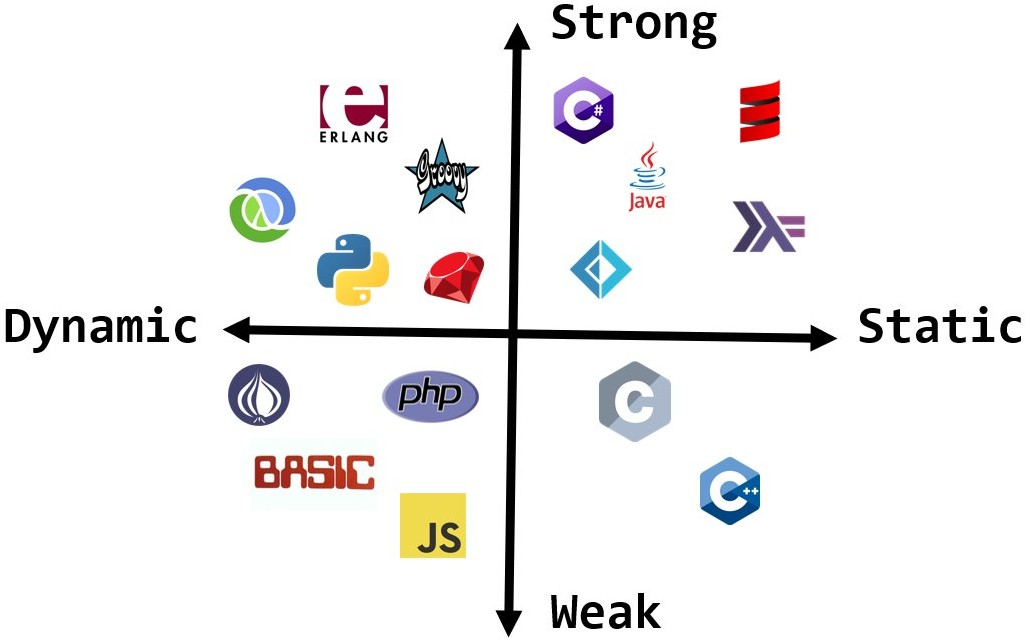
\includegraphics[width=10cm]{types.jpg}\]
\end{frame}

\begin{frame}
	\frametitle{Dynamische	vs. Statische Programmiersprachen}
	\[
		{\color{blue}\underline{\href{https://www.online-python.com/}{\text{Demonstration}}}}
	\]
\end{frame}

\begin{frame}
	\frametitle{Woher kommt Formalisierung?}
	\begin{enumerate}
		\item Erste Schritte in den 60ern und 70ern mit \textbf{Automath} und	\textbf{Logic for Computable Functions} 
		\item In den 80ern und 90ern gibt es die ersten Sprachen die breitere Anwendung finden: \textbf{Coq}, \textbf{Isabelle}, \textbf{Agda}, \textbf{PVS}
		\item Seit den 2000ern: 
		\begin{itemize}
		 \item Neue Sprachen: \textbf{Metamath}, \textbf{Lean}, ...
		 \item Formalisierung von interessanten Problemen: \textbf{Vier-Farben-Satz} (2005), \textbf{Keplervermutung} (2014), ...
		\end{itemize}
	 \item \textbf{Warum jetzt?} Benutzerfreundlicher, KI, ... 
	\end{enumerate}
\end{frame}


\begin{frame}
	\frametitle{Formalisierung im Programmieren}
	\begin{figure}
		\centering
		% First row of images
		\begin{subfigure}[b]{0.45\textwidth}
						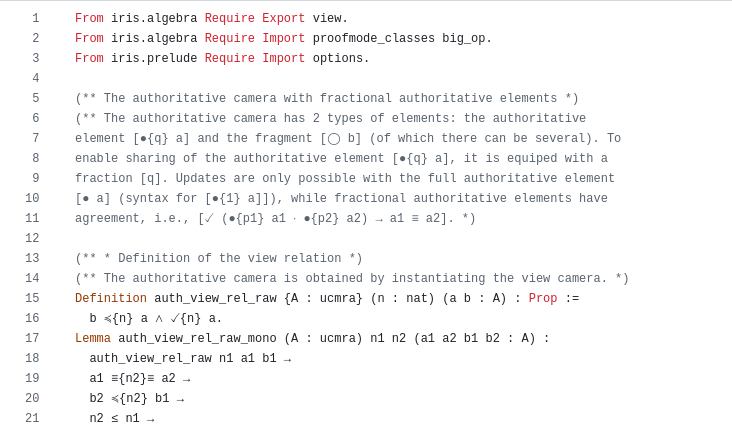
\includegraphics[width=\textwidth]{iris.png}
						\caption{\tiny \textbf{Coq} Iris}
		\end{subfigure}
		\hspace{0.5cm}
		\begin{subfigure}[b]{0.45\textwidth}
						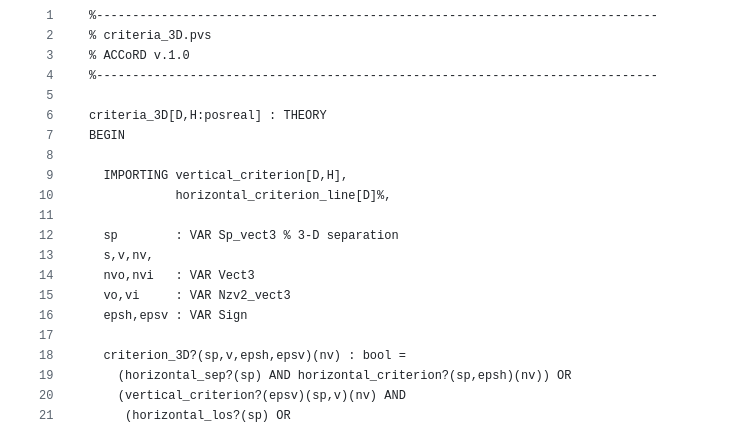
\includegraphics[width=\textwidth]{pvs.png}
						\caption{\tiny \textbf{PVS} in NASA}
		\end{subfigure}

		\vspace{0.2cm} % Space between rows
		% Second row of images
		\begin{subfigure}[b]{0.45\textwidth}
						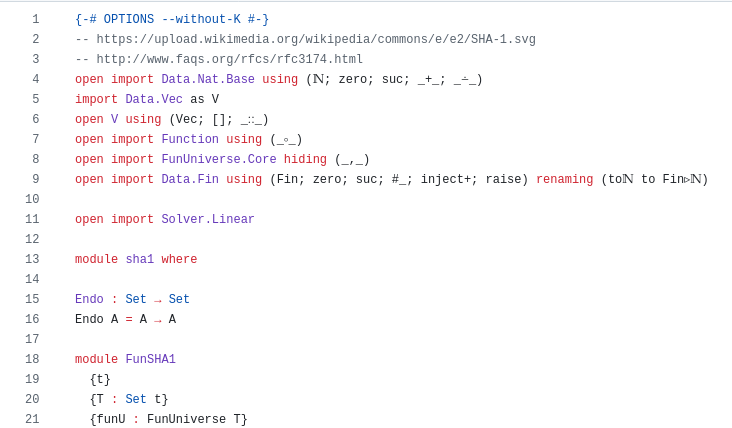
\includegraphics[width=\textwidth]{cryptoagda.png}
						\caption{\tiny \textbf{Agda} in Kryptographie $\&$ Blockchain}
		\end{subfigure}
		\hspace{0.5cm}
		\begin{subfigure}[b]{0.45\textwidth}
						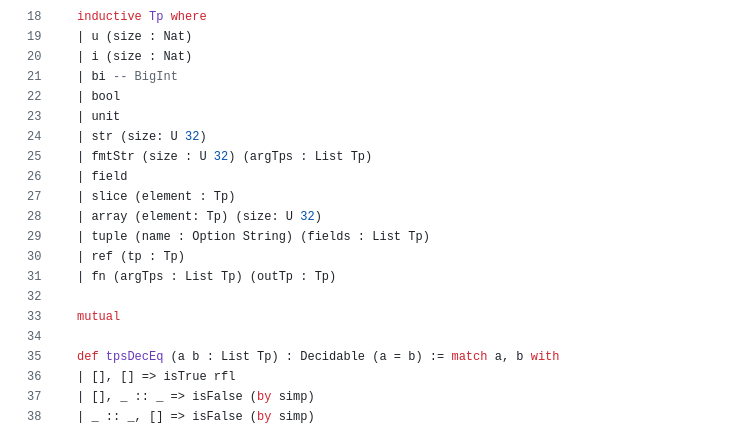
\includegraphics[width=\textwidth]{rust.png}
						\caption{\tiny \textbf{Lean} in Kryptographie}
		\end{subfigure}

\end{figure}
\end{frame}

\begin{frame}
	\frametitle{Formalisierung in der Mathematik}
 \begin{figure}
		\centering
		% First row of images
		\begin{subfigure}[b]{0.45\textwidth}
						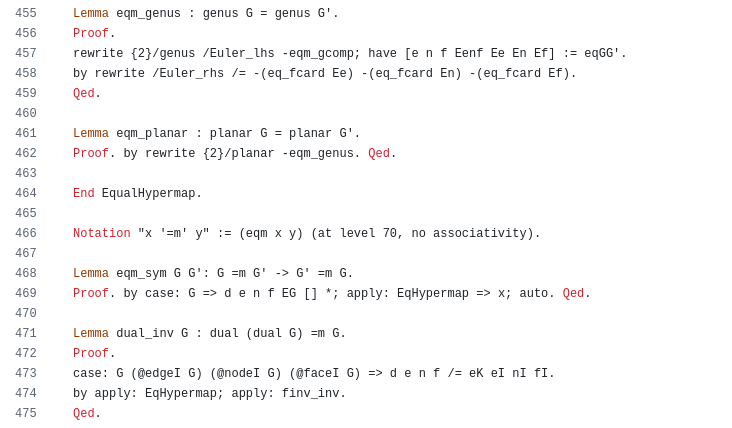
\includegraphics[width=\textwidth]{fourcolor.png}
						\caption{\tiny Vier-Farben-Satz in \textbf{Coq}}
		\end{subfigure}
		\hspace{0.5cm}
		\begin{subfigure}[b]{0.45\textwidth}
						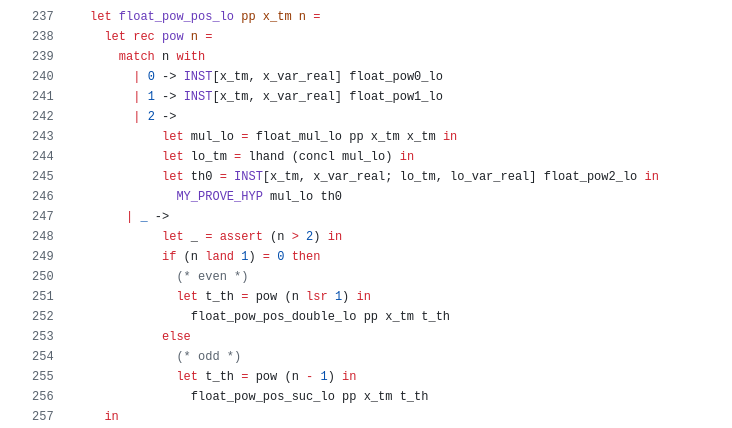
\includegraphics[width=\textwidth]{kepler.png}
						\caption{\tiny Keplervermutung in \textbf{Isabelle}}
		\end{subfigure}

		\vspace{0.2cm} % Space between rows
		% Second row of images
		\begin{subfigure}[b]{0.45\textwidth}
						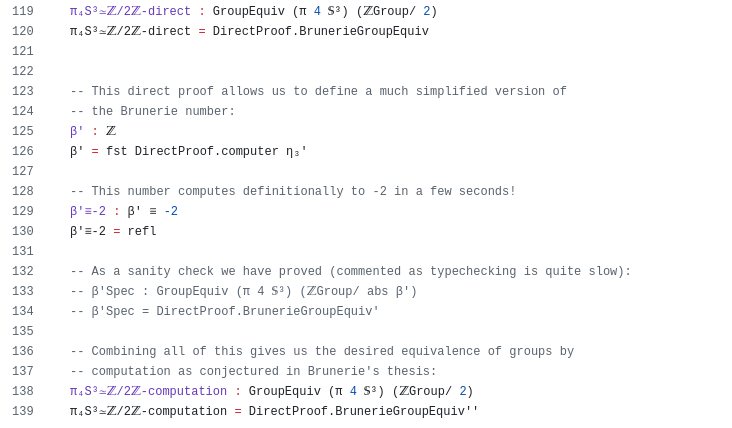
\includegraphics[width=\textwidth]{cubicalagda.png}
						\caption{\tiny Homotopiegruppen in \textbf{Cubical Agda}}
		\end{subfigure}
		\hspace{0.5cm}
		\begin{subfigure}[b]{0.45\textwidth}
						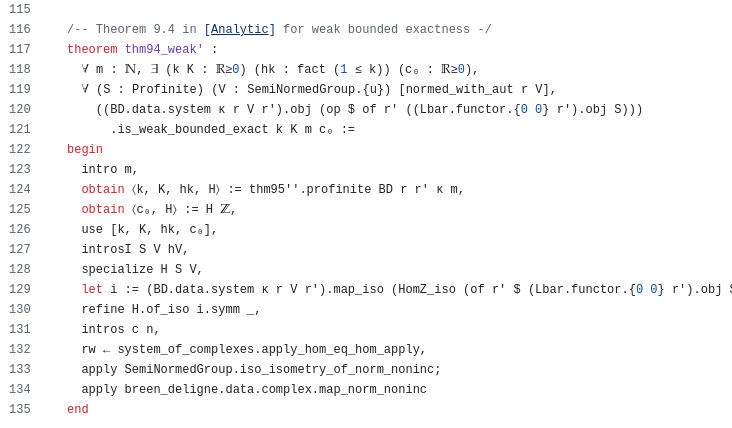
\includegraphics[width=\textwidth]{liquidtensor.png}
						\caption{\tiny Liquid Tensor Experiment in \textbf{Lean}}
		\end{subfigure}
	
\end{figure}
\end{frame}

\begin{frame}
	\frametitle{100 Probleme}
	\[
		{\color{blue}\underline{\href{https://www.cs.ru.nl/~freek/100/}{\text{Demonstration}}}}
	\]
\end{frame}

\begin{frame}
	\frametitle{Lean}
		\begin{enumerate}
			\item Wir benutzen Lean (Lean 4).
			\item Lean ist eine funktionale Programmiersprache und ein Beweisassistent.
			\item Lean wurde in 2013 von Leonardo	de Moura (erst in Microsoft, jetzt in Amazon) entwickelt.
			\item Lean 4 wurde in 2021 veröffentlicht und sollte stabil sein.
			\item Von der Struktur ähnelt es Coq 
			\item Mathematik in Lean ist in MathLib Library! 
			\item \textbf{Relativ} einfach zu benutzen	und zu lernen.
			\item Aber es \textbf{gibt} viele andere Optionen!
		\end{enumerate}
\end{frame}

\begin{frame}
	\frametitle{Lean Online}
	
	\[
		{\color{blue}\underline{\href{https://lean-lang.org/}{\text{Demonstration}}}}
	\]
\end{frame}
\begin{frame}
	\frametitle{Logik neu denken}
	\begin{itemize}
		\item In der klassischen Mathematik gibt es \textbf{Mathe} und \textbf{Logik}.
		\item \emph{Es} \emph{sei}  $f\colon S \to T$ eine \textbf{bijektive} \textbf{Abbildung} von \textbf{Mengen}. \emph{Dann} \emph{ist} $f$ \textbf{injektiv}. 
		\item \textbf{Mathe} vs. \emph{Logik}! \vspace{1cm}
	\end{itemize}
 $\Rightarrow$ Wir brauchen Mathe und Logik an einem Ort!
\end{frame}

\begin{frame}
	\frametitle{Beweise als Elemente}
	\[
		{\color{blue}\underline{\href{https://qftx.physik.hu-berlin.de/wp-content/uploads/2012/09/blackboard.jpg}{\text{Demonstration}}}}
	\]
\end{frame}

\begin{frame}
	\frametitle{Beispiele}
	\[
	\begin{tabular}{|c|c|}
		\hline 
		\textbf{Klassisch} & \textbf{Was wir wollen} \\ \hline
		Satz $P$ & $P :$ Prop \\ 
		Formel für Menge X & Abbildung f$\colon$ X $\to$ Prop \\
		Beweis für Satz $P$ & $\sigma : P$ \\
		Beweis für $P \to Q$ & Abbildung $P \to Q$ \\ 
		x = y & (x = y) ist nicht leer \\ \hline 
	\end{tabular}
	\]
	Beweis für Satz 
	\[ \exists S \forall X \forall f,g\colon S \to X (f = g)\]
 \[
	\begin{tabular}{|l|l|} \hline 
		Eine Menge S & Ein Paar $(S,\pi)$ \\
		und ein Beweis f = g & $\pi \colon (X,f,g) \to (f = g) $ \\ \hline 
	\end{tabular}
	\]
\end{frame}

\begin{frame}
	\frametitle{Beispiel in Lean}
	\[
		{\color{blue}\underline{\href{https://pathwaysmiddlecollege.org/wp-content/uploads/2023/11/image.png}{\text{Demonstration}}}}
	\]
\end{frame}

\end{document}
